
\section{Test Driven Development}

Designing code using a test first approach helps direct the design
of the code in a way that makes it more flexible. This section will
cover how to properly perform such a feat along with helpful advice
on how to handle certain aspects of the process TDD%
\footnote{Test Driven Development%
}. As such it will also explain the ways unit tests should be used
and what problems that might occur when attempting to write unit tests. 

\begin{figure}
\begin{centering}
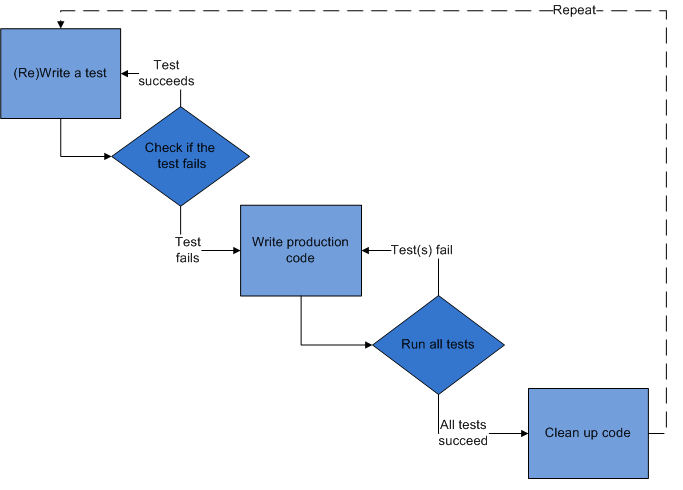
\includegraphics[width=0.7\textwidth]{TestWrittenCycle}
\par\end{centering}

\caption{The cycle of written test used to write production code (from ~\cite{WikiTDD},
\texttt{http://upload.wikimedia.org/wikipedia/en/9/9c/Test-driven\_development.PNG})\label{fig:TestWrittenCycle}}
\end{figure}



\subsection*{The Idea Behind Test Driven Development}

The idea of TDD is to write tests of how the program is supposed to
function before actually writing the program itself. These tests can
be referred to as executable specification, because they specify how
single units of the program are meant to be used.

To get an idea of how a TDD process go look at fig. \ref{fig:TestWrittenCycle},
as is shown on the fig. the idea is that you behind the development
of a unit in the program by writing a test. The test is then used
to develop the actual production code, once all tests succeed you
clean up the code and start the process is over. After multiple iterations
you ensure that not only does your code have all the features you
want, but that those features work as you would expect. Furthermore
if new features were requested at a later time it would be quite easy
to simply add new tests. 

By writing the tests first the developer can easily see how the final
program should look like, if he did not do a test first approach he
would be forced to do a lot more preplanning since he would have to
state all the specifications by them. Do not mistake however, while
a TDD approach will reduce the amount of preplanning required it will
not complete remove the need for it. It will still be required to
plan such things as the domain model and the components of the program. 

To give an idea of what the executable specification done through
TDD will show let us take this example:

Assume you were to make a Calculator, since this is a simple calculator
it can only do addition, subtraction, multiplication and division.
To specify this calculator one must create a test for each of its
features:
\begin{itemize}
\item A test showing adding two numbers 
\item A test showing subtraction of two numbers 
\item A test showing multiplication of two numbers 
\item A test showing division of two numbers
\end{itemize}
This specification will enforce that the final calculator can perform
all these actions or it will not work, thus our tests are enforcing
specified features of the calculator.

However the great thing about using TDD is that you can go deeper
and specify how the exact outcome of should be, assume that you wanted
to ensure that when the calculator divides by zero, an error is thrown.
To do this all that is required is to simply add a new test:
\begin{itemize}
\item A test showing that when the calculator divides by zero an error is
thrown.
\end{itemize}
As is evident the more tests written the more specified that aspect
of the program is, thus by doing test driven development, you have
essentially done two things at once. First you have created a way
to test if the features are still functional; this provides a way
to test them if their functionality is changed at a later date. Secondly
by making tests you are specifying what the output of the program
should be, thus if others were to try and use your units in their
code it would be easy for them to see simply by looking at the tests
you provide.


\subsection{How to write unit tests}

It is important when doing a TDD approach to properly understand how
to design unit tests, there are many problems that occur doing the
process of writing unit tests. Most of these problems can be traced
to a few common mistakes programmers do when designing a piece of
code. A good introduction to using test-driven development id Misko
Hevery's lecture on the subject, see ~\cite{LectureTDD}.

As mentioned in ~\cite{LectureTDD}, there is nothing that can be
said about writing unit tests that would improve the tests, there
is no trick to writing them. However there is a lot that can be said
about designing code, a correctly designed piece of code can make
the process of making a unit test very easy, while a badly designed
piece of code can make creating a unit test very difficult if not
impossible. To understand what these bad design choices are we will
go through each of them. 


\subsubsection*{Mixing Object creation logic with business logic}

To properly design a test for a given class in the code, you must
have access to how an object of that class gets instantiated. This
means that if the object upon instantiation create all the dependencies
it has then the test has no way to interact and as such you are forced
to not only test that class, but also all other classes this class
uses.

To give an idea of this problem assume you have a \texttt{WebDocument
}class, 

\begin{alltt}
Class WebDocument 	
    Field: Document 	
    Constructor takes URL 		
        client = new TCPClient() 		
        Document = client.Download(URL)
    Endconstructor 
Endclass
\end{alltt}

As we can see in this example the \texttt{WebDocument }creates its
own Tcp client which it uses to download from an URL. If we were to
test this class we would be forced to setup a TCP connection every
single time. This not only causes the test to be slow it also makes
it so the test becomes uncertain.

This problem can be solved by designing the class to instead of constructing
the objects itself it merely places them as requirements, this method
is called dependency injection. Going back to the \texttt{WebDocument
}example, the way it could look would be like this:

\begin{alltt}
Class WebDocument
    Field: Document 
    Constructor takes Client, URL 		
        Document = Client.Download(URL) 	
    EndConstructor 
EndClass
\end{alltt}

By making this change the test creator will have a choice, for instance
he could use a mock%
\footnote{An object that mimics the behavior of the real object%
} client. 

This basically comes down to giving choice to the unit test writer,
without this the unit tester could be required to instantiate almost
the entire program in order to just test a single unit. By using dependency
injection we effectively remove this issue.


\subsubsection*{Global State in the Code}

Whenever you have global state in your units it becomes very difficult
to design tests, as pointed out in ~\cite{LectureSingletons}. This
is because actions done in one test will inadvertently affect the
result of another test. Thus by eliminating all sources of global
state you ensure that the code which you are testing always works
in the same manner.

Most people when developing code do not even notice that they are
writing code with global state in it, this is because global state
can show up in multiple forms. By definition global state occurs every
time a piece of code knows about something that is has no reference
to thus it has reference to something that is globally accessible.

To illustrate this imagine this simple test:

\begin{alltt}
Output1 = new A().Calculate() 
Output2 = new B().Calculate() 
Assert(Output1 != Output2)
\end{alltt}

Since a computer is deterministic then that means the assertion that
the two outputs are not equal should never change. If however that
sometimes the assertion is true and other times it is false, then
we know that global state is at work. This means that global state
in code is what makes the code non-deterministic. By its very nature
code that is non-deterministic is untestable, since a test requires
knowing the outcome in advance so it can be asserted if the result
is the same.

Here we provide two examples of commonly accepted code design that
produce global state:


\subparagraph*{Singletons}

are objects is only instantiated once their instantiation is located
on a global variable, since the variable on which the singleton is
located is global, that means all objects that use the singleton has
their state bound to that of the singleton.


\subparagraph*{Random numbers, Time and date, etc.}

are all cases of objects that hides global state inside them, thus
if you use them as part of your code without providing a way for a
test to inject them as with other dependencies. Then you run the risk
of the program being untestable. The problem with these objects are
they usually hide the fact that they use global state, and as such
can easily sneak their way into the code if one is not careful. 


\subsubsection*{Breaking Law of Demeter}

One thing that makes testing difficult is if an object instead of
asking for what it needs instead asks for the object that can locate
what it needs. The act of asking only what is needed is called Law
of Demeter or principle of least knowledge. The idea is that a unit
only needs to know about its immediate friends all other units it
doesn\textquoteright{}t directly work with should be irrelevant to
it. Breaking the law of Demeter is not only considered bad code design,
but also makes writing unit test harder.

When writing code breaking law of Demeter doesn\textquoteright{}t
normally feel wrong however were we to do it in the real world the
problems with it becomes immediately visible to everyone.

As an example (adapted from ~\cite{WikiDemeter}) Imagine that you
are in a shop and the cashier asks for 10\texteuro. What would you
do?
\begin{enumerate}
\item Give him a 10\texteuro bill
\item Give him the wallet and let him find the money
\item Give him the location of a hidden treasure which he should locate
and return the difference to you.
\end{enumerate}
As we can see option 2 and 3 clearly violate law of Demeter because
instead of giving what is actually required we give something that
provides what is actually required.

In the example of the \texttt{WebDocument }we ourselves violated law
of Demeter so let us show how the code should actually look so that
the code no longer breaks law of Demeter. The code that breaks law
of Demeter:

\begin{alltt}
Class WebDocument 	
    Field: Document 	
    Constructor takes Client, URL 		
        Document = Client.Download(URL) 	
    EndConstructor 
EndClass
\end{alltt}

How the code actually should look:

\begin{alltt}
Class WebDocument 	
    Field: Document 	
    Constructor takes ADocument 		
        Document = ADocument 	
    EndConstructor 
EndClass
\end{alltt}

As we can see, instead of making \texttt{WebDocument }go locate the
document on some server instead we simply make the document a dependency
of the \texttt{WebDocument }class, thus testing of the \texttt{WebDocument
}will not even require a mock server anymore. As such designing the
test just became a lot easier.


\subsection*{Summary}

While a TDD approach will increase the workload of the project as
it will require the developer to write a lot of tests, it does so
much in return for a project. The best things about TDD it provides
specification of the programs individual units which could be hard
to properly formulate in words. Furthermore it also enforces good
code design practices this means that people in the development team
that easily succumb to making bad design decisions are stopped by
the fact that they are unable to write tests for their code.


\paragraph*{Advantages}
\begin{itemize}
\item Provides test cases for all units, making it easier to see what breaks
when units are introduced or changed
\item Reduces the amount of errors in the final product and as such reduces
time spent debugging
\item Enforce proper code design
\item Provides specification of the code making it easy for others to understand
\item Makes the writing process of a class easier since you start by stating
what you want from a class, instead of how it works.
\end{itemize}

\paragraph*{Disadvantages}
\begin{itemize}
\item Requires unit testing frameworks to do it properly
\item Has a learning curve for those no familiar with TDD
\item Increases the develop time as all code produced must also have a unit
test to prove it works as expected
\end{itemize}

\subsubsection*{References}
